\chapter{Fundamentals}  \label{Fundamentals}
  This chapter aims to give an introduction to an \ac{GNC} system as used commonly for \ac{USV} and according sensor processing algorithms to represent the \ac{GNC} systems environment. In section \ref{USV} the tasks of the three subsystems the \ac{GNC} consists of are briefly explained. Hereafter, section \ref{Quater} explains the notation for rotations as used in Unity3d. Section \ref{Houghtransf} outlines an algorithm that is used to extract lines of an image. The section is followed by an explanation of the fundamentals of distance measurement with \ac{LIDAR} in section \ref{LIDAR} and object detection with \ac{RADAR} in section \ref{RADAR}.
  
  
   \section{The \ac{USV} and Guidance, Navigation and Control} \label{USV}  
    \begin{figure}
   	\begin{centering}	
   		\begin{forest}
   			for tree={grow=0,l=3cm,anchor=west,child anchor=west} 
   			[{GNC systems}
   			[{Guidance}
   			[{Mission planning}]
   			[{Plan path}]
   			[{Update path}]]
   			[{Control actuators}]
   			[{Navigation}
   			[{Sense internal state}]
   			[{Predict future states}]
   			[{Sense environment}]]]
   		\end{forest}
   		\caption{\ac{GNC} of \ac{USV} \cite{Liu2016}.}
   		\label{fig_USVGNC}%Label für das Referenzieren 
   	\end{centering}
   \end{figure}
   Every \ac{USV} includes six basic elements which are the hull and auxiliary structural elements, propulsion and power systems, \ac{GNC} systems, communication systems, data collection equipment which are the sensors of the \ac{USV} and the ground station. According to various fields of applications, elements can be added. To operate an \ac{USV} autonomously, \ac{GNC} systems as depicted in figure \ref{fig_USVGNC} are of outstanding importance. The \ac{GNC} subsystem is divided into three main parts, namely in systems that full fill the purpose of navigation, guidance and control objectives. As these subsystems are highly interlinked with each other, a malfunction of one of them can compromise the performance of the whole \ac{USV}. 
   
   Connected to the onboard sensors, the navigation subsystem identifies future states of the \ac{USV} and represents the \ac{USV}'s current state as well as the environment. Sensors used to perceive the environment includes passive visual and infrared sensor as well as active perceptions methods such as \ac{LIDAR}, \ac{RADAR} and \ac{SONAR}. These sensors can also support the process of state estimation of the \ac{USV} as the main reference for localisation provided by the \ac{GNSS} and \ac{IMU} may be disturbed by the environmental influences. As clutter and disturbances like waves and wind are practical problems and lead to undetected targets in the application of sensors, these effects have to be filtered by appropriate methods to avoid the provision of misleading information.
   
   With the processed data of the navigation subsystem, a map with obstacles is to be generated as a first step in a so called mission planning \cite{Liu2016}. This obstacle map then allows for different methods the application of path finding algorithms to provide a trajectory from the actual position to a desired position. Two main distinctions between path planning algorithms can be made by dividing them into global and local approaches. Due to the problems of considering unexpected or dynamic obstacles when calculating a path, global approaches are more suitable for static environments or offline calculations. Further limitation in the application of these algorithms can be found in the considerably high computational resources and time to find a path. Local path finding algorithms provide the possibility of taking dynamic objects into account as they use updated sensor data and its computational effort allows real time behaviour \cite{EnvPerc}. An algorithm applying so called potential fields can be assigned to a local path finding approach. The object moves in a field of forces that originate from the kinematics of the object itself, repulsing forces of the obstacles and attracting forces from the spatial point that is to be reached. By finding a path that maximizes the potential, the object is supposed to reach the required spatial point. However, it has to be noted, that local path finding approaches are prone to find only local minima of optimal paths because they do not take into account the whole scene \cite{PotField}.
   %With the filtered information of the navigation subsystem a trajectory of the required path is planned by the guidance subsystem in a process called mission planning. The environmental conditions and the internal state and capabilities of the \ac{USV} are used to determine a trajectory which suffices the mission goals and is updated regularly according to the provided information. Different path planning methods have been proven to be feasible and can  \cite{Guidance} and are based on optimization criteria such as to find the shortest or most time efficient way to a given point \cite{EnvPerc}.
   
   With the information of both the guidance and the navigation subsystem the control subsystem determines the control forces and moments to be generated at the actuators in accordance with the desired control objectives and the \ac{USV} capabilities \cite{Liu2016}. The mathematical model to describe the ships characteristics can be sufficiently described by a three degrees of freedom model especially for inland navigation, as the ships rarely encounter large waves \cite{Control3DOF}. Therefore, the influence of heave, pitch and roll can be neglected and only the surge, sway and yaw is described by the equations of the model. Since most ships are equipped with a rudder and one or more propellers or water jets, only surge forces and the yaw momentum can be manipulated by the control system to obtain the control objectives, thus the ship model can be called under actuated. With equation \ref{eq_ControlStat} derived in \cite{ControlUnder}, the surge and yaw displacement as well as the yaw angle are described in a earth fixed frame by $x$, $y$ and $\psi$ whereas equation \ref{eq_ControlVelo} describes the surge, sway and yaw velocities by $u$, $v$ and $r$. 
  \begin{equation}
  \label{eq_ControlStat}
  \dot x= u \cos\psi- v \sin\psi, \quad \dot y= u \sin\psi+ v  \cos\psi, \quad \dot \psi= r  
  \end{equation}
  \begin{equation}
  \begin{aligned} 
  \label{eq_ControlVelo}
  & \dot u= \frac{m_{22}}{m_{11}}vr-\frac{d_u}{m_{11}}u- \sum_{i=2}^{3}\frac{d_{ui}}{m_{11}}|u|^{i-1}u+ \frac{1}{m_{11}}\tau_u+ \frac{1}{m_{11}}\tau_{wu}(t),\\
  & \dot v= \frac{m_{11}}{m_{22}}ur-\frac{d_v}{m_{22}}v- \sum_{i=2}^{3}\frac{d_{vi}}{m_{22}}|v|^{i-1}v+ \frac{1}{m_{22}}\tau_{wu}(t),\\
  & \dot r= \frac{m_{11}-m_{22}}{m_{33}}uv-\frac{d_r}{m_{33}}r- \sum_{i=2}^{3}\frac{d_{ri}}{m_{11}}|r|^{i-1}r+ \frac{1}{m_{33}}\tau_{r}(t)+ \frac{1}{m_{33}}\tau_{wr}(t)\\
  \end{aligned}
  \end{equation}
  The ships inertia as well as the added masses are denoted with $m_{xx}$ and with $d_{xx}$ the hydrodynamic damping in surge, sway and yaw is represented. Environmental disturbances are modelled with $\tau_{wu}(t)$, $\tau_{wv}(t)$ and $\tau_{wr}(t)$, caused by the influence of waves, wind and current. Higher non-linear terms are neglected to keep the model as compact as possible. The available control variables are the surge force $\tau_u$ and the yaw moment $\tau_r$. As depicted in figure \ref{fig_ControlPos}, the actual position of the ship is assumed to be specified by a point $M[x,y]$ and a direction vector $u$ which is related to the ships spatial orientation. The desired position is defined by a point $M_d[x_d,y_d]$ and a related vector $u_0$. The control objectives can be formulated by equation \ref{eq_ControlObj}. 
  \begin{equation}
  \begin{aligned} 
  \label{eq_ControlObj}
  & x_e= x_d-x, \quad y_e=y_d-y, \quad \psi_e=\psi-\psi_d \\ 
  & z_e= \sqrt{x_e^2+y_e^2}, \quad \psi_d=arcsin\frac{y_e}{z_e}\\
  \end{aligned}
  \end{equation}
	The distance difference from $M$ to $M_d$ are expressed with $x_e$ and $y_e$ which results in the summed distance $z_e$. Hereafter, the angle deviation can be formulated by $\psi_d$. Therefore, it becomes clear that in order to obtain a controllable system, the ships navigation subsystem has to provide the position and heading of the ship, the environmental data such as wind speed, the current and the waves direction as well as the scale \cite{ControlPara}. The desired state $M_d$ has to be calculated by the guidance subsystem. At least, after the computation of a suitable control, the actuators that generate the surge force and yaw moment are to be controlled accordingly \cite{ControlUnder}. 
  \begin{figure}
  	\begin{centering}
  		\begin{tikzpicture}      
  		%\draw[help lines,xstep=.5,ystep=.5,dashed] (0,0) grid (10,10); %Hilfsdiagramm für Koordinaten
  		%\foreach \x in {0,1 ,...,10} { \node [anchor=north] at (\x,0) {\x}; }
  		%\foreach \y in {0,1,...,10} { \node [anchor=east] at (0,\y) {\y}; }
  		
  		\draw[->,] (1,1) -- 	(7.5,1) node  [at end,anchor= north]{$X$}; %x axis
  		\draw[->,] (1,1) -- 	(1,7.5) node  [at end,anchor= south]{$Y$}; %y axis
  		\draw [dashed] (3,1) -- 	(3,3) node  [at start,anchor= north]{$x$}; % line to x position
  		\draw [dashed] (1,3) -- 	(3,3) node [at start,anchor= east]{$y$}; % line to y position
     	\draw[fill=black]       (3,3) circle (0.05) node (M)[below right]{$M$}; % point M
  	
  	    \draw [dashed](7,1) -- 	(7,7) node  [at start,anchor= north]{$x_d$}; % line to x_d position
  	    \draw [dashed](1,7) -- 	(7,7) node  [at start,anchor= east]{$y_d$}; % line to y_d position
  	    \draw[fill=black]       (7,7) circle (0.05) node[below right]{$M_d$}; % point M_d
  	
  		\draw[->] (3,3) -- 	(7,7) node  [midway, anchor=north]{$z_e$}; %line z_e
  		\draw[->] (3,3) -- 	(4,6) node  [midway, anchor=east]{$u$}; % line u
  		
  		\draw[->] (3,3) -- 	(7,7) node (z) {}; %line z_e to draw angles without anchor
  		\draw[->] (3,3) -- 	(4,6) node (u) {}; % line u to draw angles without anchor
         
        \coordinate (origo) at (3,3); % point M in coordinates to draw angles without anchor
        \draw [dashed](3,3) -- 	(6,3) node (y) {} ; % line to y to draw angles without anchor
  		
  		\pic["$\theta_d$" shift={(9mm,0mm)}, draw=black, <->, angle radius=1.5cm] {angle=y--origo--z};
  		\pic["$\theta$" shift={(12mm,1mm)}, draw=black, <-> ,   angle radius=2cm] {angle=y--origo--u};
  		\pic["$\theta_e$" shift={(8mm,11mm)}, draw=black, <->, angle radius=2.5cm] {angle=z--origo--u};
  		
  		\end{tikzpicture}
  		\caption{Approximation of a ships position $M$ towards a desired position $M_d$ by \cite{ControlUnder}.}
  		\label{fig_ControlPos}
  	\end{centering}
  \end{figure}
   %Insert concept of ELLA (yet classified)
   \section{Quaternions} \label{Quater}
   To describe fluid rotations of rigid bodies in a 3D space, and subsequently visualize the results in a simulation tool, a suitable mathematical representation of the rotation has to be found. Accepted as the most intuitive way are the so called Euler Angles. Rotations are described with the rotation matrix $\boldsymbol{R_{()\psi,\theta,\phi)}}$as shown in equation \ref{eq_EulerRot}. 
   \begin{equation}
   \label{eq_EulerRot}
   \boldsymbol{R_{(\psi,\theta,\phi)}} = Rot[z, \psi] Rot[x,\theta] Rot[z, \phi]  
   \end{equation}
  
   Matrix $ \boldsymbol{R_{(\psi,\theta,\phi)}}$  is composed of the three rotation $\psi, \theta, \phi$ around the three carthesian axes  $x, y, z$. However, calculating this rotation matrix and the respective rotated vector for every incremental step in order to reach a fluid rotation until a required degree is obtained is very demanding in terms of computational power. Additionally, in case one of the rotation degrees $\psi, \theta, \phi$ are zero, one degree of freedom is lost as two rotations about the same axis take place. This phenomenon is called gimbal lock. As a third back draw, the order in which the rotation about the axis are executed are important to the final result. Thus, a more suitable notation for rotations can be found in the so called quaternions. Quaternions follow a specified quaternion algebra. For instance operations on it are not commutative. Any quaternion can be written as depicted in equation \ref{eq_QuatStandard}. 
   \begin{equation}
   \begin{aligned}
   \label{eq_QuatStandard}
   & q = d + a\textit{i}+ b \textit{j} + c \textit{k} \\
   & q = cos\theta + sin\theta(s_x \textit{i} + s_y\textit{j} + s_z \textit{k} )\\
   \end{aligned}
   \end{equation}
   
   The three dimensional complex tuple $\textit{i, j, k}$ now forms a hyperspace that is in the four dimensional space that exists with the real number $\textit{d}$. $a,b,c$ or $s_x,s_y,s_z$ respectively define the rotation axis around which is rotated and represent a vector in the hyperspace as shown in figure \ref{fig_QuatHyper}. The rotation itself is defined by the angle $\theta$.  By specifying a vector $r$ as shown in equation \ref{eq_QuatVector}, the rotated vector $r'$ can be calculated with two multiplications with the normalized quaternion as in equation \ref{eq_QuatCalc} \cite{Quaternions}.
   
   \begin{equation}
   \label{eq_QuatVector}
   r = r_x\textit{i}+ r_y\textit{j} + r_z\textit{k}
   \end{equation}
   
   \begin{equation}
   \label{eq_QuatCalc}
   r' = qrq^{-1}
   \end{equation}
   
   \begin{figure}
   	\begin{centering}
   		
   		\begin{tikzpicture}      
   		%\draw[help lines,xstep=.5,ystep=.5,dashed] (0,0) grid (10,10); %Hilfsdiagramm für Koordinaten
   		%\foreach \x in {0,1 ,...,10} { \node [anchor=north] at (\x,0) {\x}; }
   		%\foreach \y in {0,1,...,10} { \node [anchor=east] at (0,\y) {\y}; }
   		\draw[->,] (3,3) -- 	(3,8)     	node (k)  [at end,anchor= south]{$k$}; % k axis
   		\draw[->,] (3,3) -- 	(1,1)     	node (i)  [at end,anchor= north]{$i$}; % i axis
   		\draw[->,] (3,3) -- 	(8,3)     	node (j)  [at end,anchor= north]{$j$}; % j axis
   		\draw[->,] (3,3) -- 	(2.5,6.5)   node (r)  [at end,anchor= east] {$r$}; % r vector	  
   		\draw[->,] (3,3) -- 	(2,5.5)   node (r') [at end,anchor= east] {$r'$};% r' vector
   		\draw[->,] (3,3) -- 	(5,2)    	node (s)  [at end,anchor= north]{$s$}; % s vector
   		
   		\end{tikzpicture}
   		\caption{A rotated vector in a Quaternion 3D hyperplane after \cite{Quaternions}.}
   		\label{fig_QuatHyper}
   	\end{centering}
   \end{figure}
  
  \section{Line Extraction with the Hough Transform} \label{Houghtransf}
   One algorithm that is widely used over time to enable a computer the extraction of patterns in images is the Hough transform. Let a greyscale  image consist of points that are defined in a two-dimensional cartesian coordinates system with some of the points fall on a line. Now given a quantity of points $X,Y$ on one line, equation \ref{Eq_Hough1} is fulfilled for the slope $m$ and intercept $b$ of that line.
   \begin{equation} 
   \label{Eq_Hough1}
   f((X,Y),(m,b)) = Y-mX-b = 0 
   \end{equation}
   Taking a single point $x,y$ separately, the lines described by the quantity of $M$ and the intercept $B$ through that point full fill equation \ref{Eq_Hough2}.
   \begin{equation} 
   \label{Eq_Hough2}
   f((x,y),(M,B)) = y-Mx-B = 0 
   \end{equation}
   The equation describes every possible line through the point $x,y$. Computing the quantity $M,B$ for several points on one line, all sets $m,b$ of values are different from each other apart from the one that describes the line on which the points lie. Because this value occurs more often, the line can be detected. The Hough transform and the line detection is visualized in figure \ref{fig_Hough1} and \ref{fig_Hough2}. With the points $a_1,a_4$ and $a_6$ in figure \ref{fig_Hough1} a line is described in the Hough image space. The image space is a picture that has been preprocessed with a edge detection with for example a Canny edge detection. For every point in the image space, the quantity $M$ and $B$ is build so that it suffices equation \ref{Eq_Hough2}. For point $a_4$ a few of the possible lines are shown. Every found combination of $m$ and $b$ is written to the Hough feature space. In the feature space, the intercept of lines is plotted against the slope. In the feature space, the line that is formed by $a_1,a_4$ and $a_6$ in the image space is plotted in black to symbolize that the corresponding slope and intercept occurs more often. Because in the feature space the values are collected that define the lines in the image space, it is called an accumulator. The more often one set of values is found, the more likely it is that a line exists in the image space.
   More precisely in the feature space, the slope and intercept is plotted in a polar coordinate system which is omitted here for reasons of simplicity. \cite{StandHough}
   
  \begin{figure}
  	\begin{minipage}[t]{0.48\textwidth}
  		\begin{centering}
  			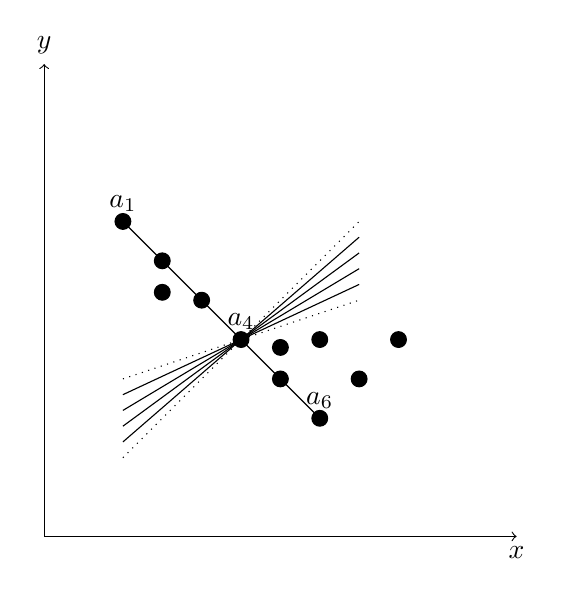
\begin{tikzpicture}      
  			%\draw[help lines,xstep=.5,ystep=.5,dashed] (0,0) grid (6,6); %Hilfsdiagramm für Koordinaten
  			%\foreach \x in {0,1 ,...,6} { \node [anchor=north] at (\x,0) {\x}; }
  			%\foreach \y in {0,1,...,6} { \node [anchor=east] at (0,\y) {\y}; }
  			
  			\draw[->,] (0,0) -- 	(6,0) node  [at end,anchor= north]{$x$}; %x axis
  			\draw[->,] (0,0) -- 	(0,6) node  [at end,anchor= south]{$y$}; %z axis
  			
  			% sorted in rising x
  			\draw[fill=black]       (1,4) circle (0.1) node (M)[above]{$a_1$}; % point M
  			\draw[fill=black]       (1.5,3.5) circle (0.1) node (M)[above right]{}; % point M
  			\draw[fill=black]       (1.5,3.1) circle (0.1) node (M)[above right]{}; % point M
  			\draw[fill=black]       (2,3) circle (0.1) node (M)[above right]{}; % point M
  			\draw[fill=black]       (2.5,2.5) circle (0.1) node (M)[above]{$a_4$}; % point M
  			\draw[fill=black]       (3,2) circle (0.1) node (M)[above right]{}; % point M
  			\draw[fill=black]       (3,2.4) circle (0.1) node (M)[above right]{}; % point M
  			\draw[fill=black]       (3.5,1.5) circle (0.1) node (M)[above]{$a_6$}; % point M
  			\draw[fill=black]       (3.5,2.5) circle (0.1) node (M)[above right]{}; % point M
  			\draw[fill=black]       (4,2) circle (0.1) node (M)[above right]{}; % point M
  			\draw[fill=black]       (4.5,2.5) circle (0.1) node (M)[above right]{}; % point M
  			
  			\draw[dotted] (1,1) --  (4,4) node []{};
  			\draw[] (1,1.2) --  (4,3.8) node []{};
  			\draw[] (1,1.4) --  (4,3.6) node []{};
  			\draw[] (1,1.6) --  (4,3.4) node []{};
  			\draw[] (1,1.8) --  (4,3.2) node []{};
  			\draw[dotted] (1,2) --  (4,3) node []{};
  			\draw[] (1,4) --  (3.5,1.5) node []{};
  			
  			\end{tikzpicture}
  			\caption{Points in image space}
  			\label{fig_Hough1}
  		\end{centering}
  	\end{minipage}\hfill
  	\begin{minipage}[t]{0.48\textwidth}
  		\begin{centering}
  			\begin{tikzpicture}      
  			%\draw[help lines,xstep=.5,ystep=.5,dashed] (0,0) grid (6,6); %Hilfsdiagramm für Koordinaten
  			%\foreach \x in {0,1 ,...,6} { \node [anchor=north] at (\x,0) {\x}; }
  			%\foreach \y in {0,1,...,6} { \node [anchor=east] at (0,\y) {\y}; }
  			
  			\draw[->,] (0,0) -- 	(6,0) node  [at end,anchor= north]{$m$}; %x axis
  			\draw[->,] (0,0) -- 	(0,6) node  [at end,anchor= south]{$b$}; %z axis
  			
  			
  			% sorted in rising x
  			\draw[fill=black]       (1.5,3) circle (0.1) node (M)[above]{$c_1$}; % point M
  			\draw[]       (1,3.5) circle (0.1) node (M)[below right]{}; % point M
  			\draw[]       (0.5,4) circle (0.1) node (M)[below right]{}; % point M
  			\draw[]       (3,2) circle (0.1) node (M)[below right]{}; % point M
  			\draw[]       (1.7,2.5) circle (0.1) node (M)[below right]{}; % point M
  			\draw[]       (3,2.7) circle (0.1) node (M)[below right]{}; % point M
  			\draw[]       (14,2.4) circle (0.1) node (M)[below right]{}; % point M
  			\draw[]       (1.8,1.5) circle (0.1) node (M)[below right]{}; % point M
  			\end{tikzpicture}
  			\caption{Lines in feature space}
  			\label{fig_Hough2}
  		\end{centering}
  	\end{minipage}
  \end{figure}
  
   \section{Distance Measurement with \ac{LIDAR}} \label{LIDAR}
   With the rapid development of lasers for optical distance measurement, today the \ac{LIDAR} technology is widely used in different fields of applications. After an introduction to the working principle of a \ac{LIDAR}, this section continuous by detailing four clustering algorithms that can be applied on the \ac{LIDAR} data. In subsection \ref{Hough3d} the Hough algorithm for the three-dimensional space is explained followed by the partition based K-Means algorithm in subsection \ref{K-means}. Hereafter, subsections \ref{Birch} and \ref{DBSCAN} explain the hierarchic \ac{BIRCH} and density based \ac{DBSCAN} algorithm respectively.\\
   
   A classification based on the transmission waveform and data processing method divides the \ac{LIDAR} technology into pulsed, continuous wave, pulse compression, moving target display, pulse Doppler and imaging \ac{LIDAR}. All of these varieties are based on the fundamental principle of a \ac{LASER}. The wavelength of the laser is in the range of ultraviolet, infrared or visible light. Typically, a wavelength of about 1000nm or less is used. One advantage that a pulsed laser has over a continuous laser is the higher light intensity for a period of time. A typical measurement cycle according to the pulsed laser method comprises three integrations. A laser pulse is emitted and the received radiation is registered via integration one. After the time $t_{pulse}$ is elapsed, in the first integration the backlight and the first part of the reflected pulse is saved. Hereafter, integration two sums up the backlight and the last part of the reflected pulse. Integration three solely measures the backlight over a certain period of time. With equation \ref{Eq_ToFdirekt2} derived in \cite{ASpieck} and in \cite{ADrie}, the quotient $Q_{ToF}$ can be calculated. The backlight or noise is subtracted by integration three from the reflected light measured in integration one and two. With the pulse length $t_{pulse}$, $t_{ToF}$ can be calculated by \eqref{Eq_ToFdirekt3}. By multiplication with the speed of light $c$, the now known value  $t_{ToF}$ results in the distance of the object from which the light was reflected.
      
    \begin{equation} 
   \label{Eq_ToFdirekt2}
   Q_{ToF}=\frac{integration2-integration3}{integration1+integration2-2*integration3}
   \end{equation}
   
   \begin{equation}
   \label{Eq_ToFdirekt3}
   t_{ToF}=t_{pulse}*Q_{ToF}
   \end{equation}
   
   \begin{equation} 
   \label{Eq_ToFdirekt1}
   d=\frac{c}{2}*t_{ToF}
   \end{equation}                                                                                                                               
   To obtain a point cloud and scan the environment of the \ac{LIDAR}, the emitted light has to be directed by some means. Different scanning methods exist of which one is a motor-driven rotation of a mirror, which reflects the laser and hereby allows sampling of the surrounding of up to 360\degree. As moving parts are part of this method, friction and therefore a reduced durability are inherent to this approach. However, because of the technical simplicity this implementation is widely used. A typical mechanical \ac{LIDAR} scanner with the aforementioned laser as a source, comprises the a servo motor as an actuator and a mirror as the rotational element.
  
   
   The segmentation of the \ac{LIDAR} data takes a vital role to extract the necessary information used for the subsequent object classification.  A number of segmentation algorithms were proposed in the last years which can be divided into direct and indirect approaches. Given a point cloud with artefacts shaped in regular geometric shapes, an example for a direct
   approach is given by the Hough transformation. Geometric parameters can be extracted directly from the point cloud data besides the segmentation process. Indirect segmentation methods apply for example progressive algorithms (over time improving approximations of a complete solutions with intermediate results \cite{ProgAlg}) on the point cloud data to compute spatial proximity and geometric derived values as for example local surface normal vectors. Common algorithms for an indirect data segmentation by clustering without feature extraction comprise methods based on partitioning, hierarchy and density. 
   
   \subsection{Hough Transform Algorithm (direct approach)} \label{Hough3d}
   The Hough Transform Algorithm for the 3D space works similar to the Hough Transform Algorithm in the 2D space which is frequently used in image feature extraction. The 2D Hough algorithm is explained in section \ref{Houghtransf}. Let a planar feature in the 3D carthesian space be described by a function F as shown in equation \ref{eq_imSpace}, it can be converted into angle information to the form in equation  \ref{eq_featSpace}.
   \begin{equation} 
   \label{eq_imSpace}
   F=ax+ by+ cz+ d= 0%\frac{c}{2}*t_{ToF}
   \end{equation} 
  \begin{equation}
   \begin{aligned} 
   \label{eq_featSpace}
    &\rho= x\cos\theta\sin\phi+ y\sin\theta\sin\phi+ z\cos\phi \\
    & \theta \in [0\degree,360\degree], \phi \in [-90\degree,90\degree]
   \end{aligned}
   \end{equation}
   
   The normal vector n of the planar feature is described by the parameters $\theta, \phi$ and $\rho$ as depicted in figure \ref{fig_HoughIm}. Accordingly, the Hough space consist of these parameters. The algorithm (accumulator) now iterates through the point cloud data and maps the possible normal vectors of each point in its feature space
   (Hough space). Hence, every time a point is on the planar feature, the density of the parameters ($\theta, \phi, \rho$) in the feature space related to n will increase. Points with a high density in the feature plane therefore represent a plane in the 3D carthesian space and the feature is extracted. However, for each point in data, there are 
   $x_\theta*x_\phi$ possibilities to be mapped in the feature space. With $y$ points in the point cloud the accumulator needs $y*x_\theta*x_\phi$ iterations to finish the process. For large databases, the process therefore requires many iterations and the computational power has to be sufficient to cluster the database in the required time frame of the application.
   \begin{figure}
   	\begin{centering}
   		\begin{tikzpicture}      
   		%\draw[help lines,xstep=.5,ystep=.5,dashed] (0,0) grid (10,10); %Hilfsdiagramm für Koordinaten
   		%\foreach \x in {0,1 ,...,10} { \node [anchor=north] at (\x,0) {\x}; }
   		%\foreach \y in {0,1,...,10} { \node [anchor=east] at (0,\y) {\y}; }
   		\draw[->,] (3,3) -- 	(3,8)     	node (z) [at end,anchor= south]{$z$}; %z axis
   		\draw[->,] (3,3) -- 	(1,1)     	node (x) [at end,anchor= north]{$x$}; %x axis
   		\draw[->,] (3,3) -- 	(8,3)     	node[at end,anchor= north]{$y$}; % y axis
   		\draw[->,] (3,3) -- 	(4,7.5)   node (n)[midway,anchor= east]{$\rho$} node[at end,anchor= east]{$n$}  ; % n axis normal vector to plane		  
   		\draw[] (4.5,5) -- 	(7.5,6)   	; % plane line
   		\draw[] (4.5,5) -- 	(2,6)     	; % bottom to right plane line
   		\draw[] (2,6) -- 	(4.5,7)     	; % bottom to left plane line
   		\draw[] (4.5,7) -- 	(7.5,6)     ; % mid to top plane line
   		\draw[dashed] (3,3) -- (3.75,2) node (xy)[] {} ; % bottom square intersecting line 
   		\draw[dashed] (2,2) -- (3.75,2) ; % bottom square left to right
   		\draw[dashed] (4.75,3) -- (3.75,2)     ; % bottom square right to top
   		\draw[dashed] (3.75,6.5) -- (3.75,2)     ; % %perpendicular to bottom suquare to plane
   		%\coordinate at (5,6.5) node {P};
   		\coordinate (origo) at (3,3); % origin coordinates coordinate system
   		\pic[draw, "$\phi$", angle radius=0.5cm, anchor= south west] {angle=xy--origo--n}; %angle phi
   		\pic[draw, "$\theta$", angle radius=0.7cm] {angle=x--origo--xy}; % angle theta
   		\end{tikzpicture}
   		\caption{A planar feature described in the 3D hough image space \cite{EnvPerc}.}
   		\label{fig_HoughIm}
   	\end{centering}
   \end{figure}

   \subsection{K-Means algorithm (partition based) }  \label{K-means}
   The K- means partitioning algorithm follows a very straight forward method and is divided into three steps. The first step is to find a center point for each cluster, which can be done randomly. The distance from each point to the center point of each cluster is calculated in a second step. In a third step, the average coordinates from each point of a cluster is calculated and defined as the new center of the according cluster. Step two and three can be iterated until a difference criterion between the former and actual cluster center is found. Therefore to reach a certain accuracy, many iterations can be necessary and the computational effort for large databases is high.
   \subsection{BIRCH Algorithm (hierarchic)} \label{Birch}
   The \ac{BIRCH} algorithm is used for very large datasets which are to be processed in a limited time with very small amount of used memory space. In most cases, one single scan of the data which is to be clustered is sufficient. Furthermore, noise is handled effectively \cite{BIRCH}.
   Based on the \ac{CF} and the hierarchical \ac{CFT}, the \ac{CF} is  defined by the triplet $(N_i, \vec{LS}, \vec{SS})$, in which $N_i$ represents the $i$ data points in the cluster, $\vec{LS}$ the sum $\sum N_i$ and $\vec{SS}$ the sum of squares $\sum N_i^2$. The cluster features can be added to each other which is expressed by equation \ref{eq_BirchMerge}.
   \begin{equation}
   \label{eq_BirchMerge}
   CF1+CF2=(N1+N2, \vec{LS1}+\vec{LS2}, \vec{SS1}+\vec{SS2})
   \end{equation}
    The \ac{CF} are stored in a \ac{CFT} with Root, Nonleaf, and Leafnotes and the MinCluster as depicted in figure \ref{fig_BIRCHTree}. B describes the maximum branches of the Nonleafes and L the maximum branches of the MinCluster. The parameter T limits the radius of the cluster. The algorithm consists of five consecutive steps. First, the nearest CF node to the new sample is found. If, second, the distance between the new sample and the CF node is less than the threshold T, insert the sample. Otherwise, and if the CF branches (MinCluster) of the leaf node are below the threshold L, insert a new MinCluster. If the threshold requirement L is not met, in a fourth step divide the leaf into two new leafs. The two MinCluster furthest away from each other are selected for the new leaf nodes. The new sample and the already given samples have to be assigned to the according leaf hereafter.
   
   The main advantage is that no iteration over the datapoints is necessary, as each datapoint is read in only once. As the \ac{CFT} only points to the data that is saved, even high amounts of data can be processed. However, due the limited \ac{CF} per node, the algorithm is prone to over segmentation and is also called a micro clustering approach. Therefore, created cluster may not represent the real world situation especially for large target objects in the measured data \cite{EnvPerc}. Additionally due to distance restriction of the \ac{CF}, the shape of the cluster data tends to be spherical for large target objects.
 
\begin{figure}
	\begin{centering}
	
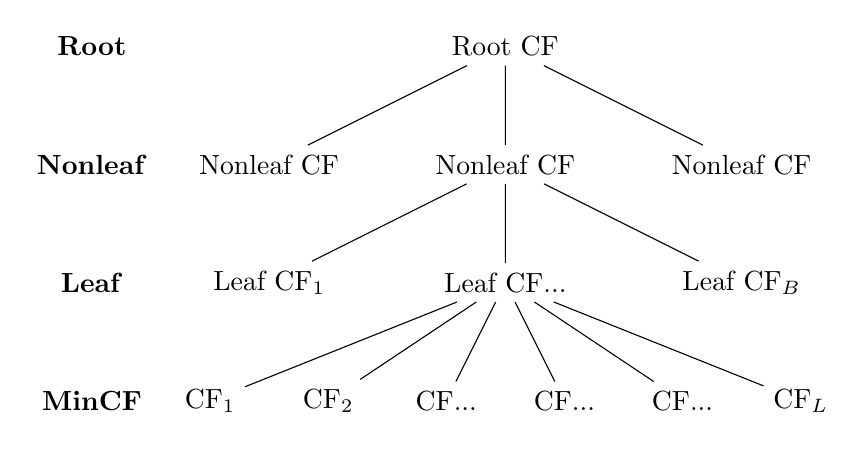
\begin{tikzpicture}[level distance=1.5cm,
level 1/.style={sibling distance=3cm},
level 2/.style={sibling distance=3cm},
level 3/.style={sibling distance=1.5cm},
level 4/.style={sibling distance=1cm}]

\node (Root) {Root CF} % Root cluster
child {node {Nonleaf CF}} % nonleaf cluster
child {node {Nonleaf CF}  % nonleaf cluster
	child {node {Leaf CF$_1$}} % leaf cluster
	child {node {Leaf CF...} % The CF nodes start below this Leaf CF
		child {node{CF$_1$} % From this node, the level describtion starts from downwards to Root
			child [grow=left] {node (q) {\textbf{Min\ac{CF}}} edge from parent[draw=none] % level description Cluster
				child [grow=up] {node (q) {\textbf{Leaf}} edge from parent[draw=none] % level description Nonleaf
					child [grow=up] {node (q) {\textbf{Nonleaf}} edge from parent[draw=none] % level description Leaf
						child [grow=up] {node (q) {\textbf{Root}} edge from parent[draw=none]}}}}} % level desctiption Root
		child {node{CF$_2$}} % cluster CF
		child {node{CF...}} % cluster CF
		child {node{CF...}} % cluster CF
		child {node{CF...}} % cluster CF
		child {node{CF$_L$}}}	% cluster CF
	child {node {Leaf CF$_B$}}} % cluster CF
child {node {Nonleaf CF}}% non leaf CF
;
\end{tikzpicture}
\caption{A \ac{CFT} derived from the \ac{BIRCH} Algorithm \cite{EnvPerc}.}
\label{fig_BIRCHTree}%Label für das Referenzieren 
\end{centering}
\end{figure}
\subsection{DBSCAN (density based)} \label{DBSCAN}
With the \ac{DBSCAN} algorithm a method is proposed with which arbitrary shaped targets can be clustered even in an environment with present noise. It is a density based approach and efficient for large spatial databases. The algorithm takes advantage of the characteristic of a shape or cluster, that the points of the cluster provide a higher density than the noise outside of a cluster. Therefore each point inside a cluster requires to have a minimum of points $MinPts$ inside its neighbourhood $Eps$. The shape of a neighbourhood is to be determined by the function of distance of two points with $dist(p,q)$, where $Eps$ is the maximum distance between two points $p,q$ to consider them as neighbours. For example for an Euclidean distance the shape of a neighbourhood would be spherical and for a Manhattan distance, the shape would be rectangular. Equation \ref{eq_DBSCANDef1} describes this relation with $N_{Eps}$ describing the $Eps$ neighbourhood and $D$ the dataset of points in a k-dimensional space to be considered.
 \begin{equation}
\label{eq_DBSCANDef1}
N_{Eps}(p)= \{q\in D |dist(p,q) \leq Eps \}
\end{equation}
A point $p$ that full fills the requirement of $MinPts$ points $q$ in its neighbourhood is considered to be directly-density-reachable with the formal definition described by equation \ref{eq_DBSCANDef2}.
\begin{equation}
\label{eq_DBSCANDef2}
p \in N_{EPS}(q) \land |N_{Eos}(q)| \geq MinPts
\end{equation}
However, because a data point $p$ at the border of a cluster may not full fill the requirement of $MinPts$ points inside its neighbourhood but is nevertheless inside the cluster, its relation to a point $q$ is defined by the expression density-reachable. A point $p$ is density-reachable, if there is a chain of points $p_1,...,p_i= q, p_n=p$ with $p_{i+1}$ directly-density-reachable from $p_i$. A third definition is required to describe the relation of two points $p$ and $q$ both at the border of a cluster. They are density-connected if a point $o \in N_{Eps}$ is density-reachable from $p$ and $q$ \cite{DBSCAN} \cite{DBSCANRev}. Figure \ref{fig_DBSCAN} depicts the aforementioned relations with the points B, A, C and N. N can be considered as noise and is unrelated to a cluster because it is not connected to another points by any given definition. The data points A are directly-density-reachable from each of the red points. The data points B and C are density-reachable from A and the other red points are density-connected to each other by the red points. The found cluster now consists of the red and yellow points.

As density based algorithms as the \ac{DBSCAN} depend essentially on the closeness $Eps$ of the data points to each other, spatially distributed cluster and varying density results in large inaccuracies \cite{ClusterOver}. Therefore, in an environment with these characteristics an adaptive value for $Eps$ is required. A linear threshold expressed with equation \ref{eq_DBSCANAdv} has been experimentally proven to be feasible. The arc length $L$ is calculated with the angle resolution $\theta$ and the distance $d_i$ and results in $Eps$ together with the precision factor $n$. Additionally, because not only the distance of points to each other, but the density of points inside a cluster can be reduced by increasing distance, the minimum of required points inside a cluster may be adapted with a linear equation related to the distance \cite{AdvancedDBSCAN}.
\begin{equation}
\begin{aligned} 
\label{eq_DBSCANAdv}
& L= \frac{\theta\pi d_i}{180}  \\
& Eps = nL
\end{aligned}
\end{equation}

 
   
   \begin{figure}
   	\begin{centering}
   		\includegraphics[width=0.5\linewidth,keepaspectratio]{Bilder/DBSCAN.png}
   		\caption{Clustered data with \ac{DBSCAN} and noise \cite{DBSCANRev}.}
   		\label{fig_DBSCAN}%Label für das Referenzieren 
   	\end{centering}
   \end{figure}
   
   
   \section{Object Detection with \ac{RADAR}} \label{RADAR}
   After an introduction to the fundamental formulas that describe \ac{RADAR} systems, this section continuous with four different approaches to filter the \ac{RADAR} data. in subsection \ref{constThresh}, a constant threshold is explained to separate noise from the signal. Continued by subsection \ref{CFARthr}, a dynamic threshold calculation is introduced which is the foundation for subsection \ref{OSthre} and \ref{SOCAthre}. In this subsections, derivatives to the afore mentioned dynamic threshold calculation are explained.\\  
   
   A millimetre wave \ac{RADAR} can estimate distances by means of electromagnetic waves with a frequency between 30GHz and 300GHz and wavelength between 1-10mm. An electromagnetic wave is emitted and reaches a possible target with the energy $S_e$ (equation \ref{eq_RADAREmit}). In equation \ref{eq_RADAREmit}, $g$ represents the antenna gain, $P_S$ the power of emittance in Watts and $r$ the distance from the antenna to the target.  
   \begin{equation}
   \label{eq_RADAREmit}
   S_e=\frac{gP_s}{4\pi r^2} \quad \quad  [\frac{W}{m^2}] % quad for spacing
   \end{equation}
   The electromagnetic wave is then reflected with the energy $S_s$ according to equation \ref{eq_RADARRec} with $r$ similar to \ref{eq_RADAREmit} and $A_e$ being the RADAR cross section calculated by \ref{eq_RADARCross} \cite{Funk}. 
   \begin{equation}
   \label{eq_RADARRec}
   S_s=\frac{A_eS_e}{4\pi r^2} \quad \quad  [\frac{W}{m^2}]
   \end{equation}
   Equation \ref{eq_RADARCross} can be described as the ratio of the target surface $A_{pl}$ to the wavelength $\gamma$ of the emitted wavelength. Therefore, the larger the wavelength and the smaller the surface area of the target object, the smaller the reflected energy and the higher the signal to noise ration. For practical considerations, in most cases values with sufficient accuracy can be calculated by approximating the target area as planar\cite{Funk}. For further specification, the power of the radiation depends on the size, shape and material of the target \cite{EnvPerc}.
   \begin{equation}
   \label{eq_RADARCross}
   A_e=4\pi\frac{A_{pl}^2}{\gamma^2} \quad \quad  [m]
   \end{equation}
   
   Two operational principles can be distinguished of which the first is the continuous wave system RADAR and the second the pulse system RADAR. In the continuous wave system the reflectance of the target object is received during the emittance of waves. In the pulsed system, a wave is emitted intermittently and during the emittance breaks, the reflectance is received. Inherent to both systems is the importance of signal processing to increase the target detection in a non uniform environment and improve target position estimation. 
   
   \subsection{Constant Threshold} \label{constThresh}
   The most straight forward approach is to empirically determine a threshold to separate the objects reflectance signal from the noise and clutter of the measurement. The higher the threshold, the lower the probability of false alarms becomes. However, with a high threshold, the probability to ignore targets becomes higher, too. Therefore, the level of the threshold is vital in this approach. To add further robustness, several measurements of the same object can be compared and only data points which are consistently above the threshold can be specified as an object representation. Hence, the more measurements are made, the higher is the certainty with which objects can be determined. In figure \ref{fig_ConseqRADAR}, four different measurements of the same scene are depicted. On the first axis the time $t$ is plotted and the second axis represents the reflected signal strength $U_E$. Only the corresponding value of $t_x$ to $t_x+\Delta t_x$ is above the threshold $U_S$ in all measurements. Thus, a target reflectance can be associated to this period of time with some certainty. In contrast, the time $t_y$ to $t_y+\Delta t_y$ exceeds the threshold only once and can be classified as noise or clutter \cite{Funk}. Due to the fixed threshold, environments with changing noise intensity results in varying probabilities for false alarms. Additionally, the targets reflectance may change due to positional deviations and resulting surface area changes and thus further raise the false alarm probability. 
   \begin{figure}
   	\begin{centering}
   		\includegraphics[width=5cm,keepaspectratio]{Bilder/ConseqRADAR.png}
   		\caption{Four datasets to distinguish the target from noise and clutter \cite{Funk}.}
   		\label{fig_ConseqRADAR}%Label für das Referenzieren 
   	\end{centering}
   \end{figure}
       
   \subsection{\ac{CFAR}} \label{CFARthr}
    By taking the \ac{SNR} as a threshold rather than the absolute value of the signal, an adaptive signal threshold can be realized and the probability for an false alarm is reduced even in situations with a high noise signal strength. First, the noise of the measurement has to be determined and normalized. Specifically in naval applications, the noise can be approximated with different \acp{PDF} of which one is the Rayleigh distribution \cite{SeaClutter}. The \ac{PDF} of the Rayleigh distribution is shown in equation \ref{eq_Ray} with the noise $x$ and $b$ proportional to the mean of the noise $\mu$ according to \ref{eq_RayFac}.  
   \begin{equation}
   \label{eq_Ray}
   P(x)=\frac{x}{b}^{-\frac{x^2}{2+b^2}}
   \end{equation}
   \begin{equation}
   b=\sqrt{\frac{2}{\pi}}+\mu
   \label{eq_RayFac}
   \end{equation}
   To express equation \ref{eq_Ray} independent of the noise level, $b$ can be substituted by $y=x/b$ which results in equation \ref{eq_RayUn}. \begin{equation}
   \label{eq_RayUn}
   P(y)=y^{-\frac{y^2}{2}}
   \end{equation} 
   The probability for a value $y$ is now only dependent on the \ac{SNR} of the target signal to the mean noise of the environment. A system diagram of the necessary operations is provided by figure \ref{fig_CFAR}. A mean value $\mu$ of the noise is calculated with one or more sampling pulses and compared with the input signal $x$. It is not required to take additional sampling pulses to the already taken samples, because the noise can be extracted from the present measurements. This can be either done by dividing the area of interest into cells and measure the noise in cells surrounding the target by assuming that these cells only consist of noise \cite{SigProcRADAR}. Another approach is to use the measured signal levels before and after the target reflectance. Therefore, it has to be assumed that the area before and after the target represents solely noise \cite{EnvPerc}. After the noise extraction, the mean value $\mu$ of the noise is estimated and compared to the input signal $x$. The hereby resulting value $y$ is given to the detector, which compares the value to the  \ac{SNR} threshold $U_0$. Either the signal is above the determined threshold and the output results in a target signal (one) or the threshold is not exceeded and therefore no target signal is detected (zero). The probability for a false alarm therefore can be set through the threshold.
   \begin{figure}
   	\begin{centering}
   		\includegraphics[width=0.75\linewidth,keepaspectratio]{Bilder/CFAR.png}
   		\caption{Single target \ac{CFAR} with fixed threshold  \cite{EnvPerc}.}
   		\label{fig_CFAR}%Label für das Referenzieren 
   	\end{centering}
   \end{figure}
  
   
   \subsection{\ac{OS-CFAR}} \label{OSthre}
   Considering the possibility of different noise and clutter levels in the sample, the aforementioned method with a very basic noise calculation approach can reach its limits in real world applications. The method as proposed in \cite{AdvCFAR} resembles the ideas of image processing. More specific, the clutter and noise power estimation that for example derives one value by averaging the whole noise sample is replaced by an arithmetic averaging procedure that is applied already in image processing applications. Especially for dense target situations, the proposed method provides advanced target extraction capabilities. The most significant change to common \ac{CFAR} approaches is the application of order statistics to derive a noise value close to the field of interest. The field of interest is divided into cells of which the centre cell is called \ac{CUT} as depicted in figure \ref{fig_StatCFAR}. The aim is the decision whether there is a target present in the cell or not by comparing the signal strength of the cell with its surrounding cells. The green cells right and left of the \ac{CUT} are called guard cells and are lined up in a one dimensional space in this example. In a three dimensional application they would build a sphere around the \ac{CUT} accordingly. They are ignored in the measurement, because the signal energy can affect adjacent cells and may effect the noise calculation. The signal strength of the cells $x_1...x_N$ and $y_1...y_M$ are most important for the noise calculation and are processed by the order statistic process in such a way that $x_{(1)}\leq... \leq x_{(k)}\leq... \leq x_{(N)}$ and $y_{(1)}\leq... \leq y_{(k)}\leq... \leq y_{(N)}$. Hereafter, these values can be described by a \ac{PDF} of order statistics. One value $x_k, \quad k \in \{1,2,...,N\}$ or $y_k, \quad k \in \{1,2,...,M\}$ is then selected and used as an estimation for the average noise power $Z$ as shown in equation \ref{eq_AvClut}.
   \begin{equation}
   Z= X_{(k)}
   \label{eq_AvClut}
   \end{equation}
   By scaling $Z$ with the factor $T$, an adaptive threshold $S$ for the comparator is found (equation \ref{eq_thres}). 
   \begin{equation}
   S= TZ
   \label{eq_thres}
   \end{equation}
   In figure \ref{fig_StatCFAR}, $\alpha$ resembles the scaling factor $T$ of equation \ref{eq_thres} and with $\beta$ the threshold can be further adjusted. A comparator thereafter compares the value of the \ac{CUT} to the threshold and the decision is made, whether there is a target (one) or only noise (zero) in the according cell. The algorithm then iterates through the cells until each cell is set to zero or one. The advantage of multi target detection in this approach resulting from the independency of the mean value of the clutter comes by the disadvantage of high computational effort to calculate the threshold. The probability that a random noise variable $Y_0$ of the \ac{CUT} is interpreted as an echo of the target can be expressed with equation \ref{eq_OrdStat}. To obtain a required false alarm rate, this equation has to be solved to derive the scaling factor $T$. 
   \begin{equation}
   P_{fa}=P[Y_0\geq TZ]
   \label{eq_OrdStat}
   \end{equation}
   As aforementioned, in sea borne applications, the Rayleigh function can be used as an estimation to clutter and therefore describes the \ac{PDF} of $Y_0$ sufficiently. However to proof the independency of the mean value of all noise values in the threshold calculation, a simple exponential distribution for the noise following $1/\mu e^{-x/\mu}$ is sufficient. The \ac{PDF} of $Z=x_k$ is shown by equation \ref{eq_OrdEq}.
   \begin{equation}
   P_{x_k}= \frac{k}{\mu_{N,k}}{e^{\frac{-x}{\mu}}}^{N-k+1}({1-e^{\frac{-x}{\mu}}}^{k-1})
   \label{eq_OrdEq}
   \end{equation}
   As both \ac{PDF} of $Y_0$ and $Z=x_{(k)}$ are known, the scaling factor $T$ can be calculated for a required false alarm rate $P_{fa}$ with equation \ref{eq_OrdStat} which results in equation \ref{eq_OrdP}.
   \begin{equation}
   P_{fa}= k_{N,k}\frac{(k-1)!(T+N-k)!}{(T+N)!}
   \label{eq_OrdP}
   \end{equation}
   It has to be noted that with this equation, the probability for a false alarm no longer depends on the mean value $\mu$ but solely on the scaling factor $T$ the fixed value $N$ or $M$ describing the number of the sample cells and the sample index $k$. For a fixed false alarm rate the literature proposes values for the threshold $T$ to limit the computational effort to derive these values \cite{AdvCFAR}.
	\begin{figure}
		\begin{centering}
			\includegraphics[width=0.6\linewidth,keepaspectratio]{Bilder/StatCFAR.png}
			\caption{Multi target \ac{OS-CFAR}, threshold calculated by ordered statistics \cite{SigProcRADAR}.}
			\label{fig_StatCFAR}%Label für das Referenzieren 
		\end{centering}
	\end{figure}
 
    \subsection{\ac{SOCA-CFAR}} \label{SOCAthre}
   The \ac{SOCA-CFAR} algorithm is a variation of the \ac{CFAR} algorithm and takes the lowest mean value of the cells right and left to the \ac{CUT} \cite{SigProcRADAR}. Therefore, the chance to detect targets with low energy is high and the computational effort moderate. That comes with the back draw of a higher false alarm detection rate. In figure \ref{fig_SOCACFAR} the difference to other algorithms that are based on the \ac{CFAR} method becomes clear with the orange box that decides in favour of the lowest mean value of $x_i$ and $y_i$. This is expressed by equation \ref{eq_SOCA}.% The other variables in the figure resemble figure \ref{fig_StatCFAR}. 
   
   
   
   \begin{equation}
   Z= \min (\frac{1}{N}\sum_{i=1}^{N}x_i,\frac{1}{M}\sum_{i=1}^{M}y_i)
   \label{eq_SOCA}
   \end{equation}
   
   \begin{figure}
   	\begin{centering}
   		\includegraphics[width=0.6\linewidth,keepaspectratio]{Bilder/SOCACFAR.png}
   		\caption{\ac{SOCA-CFAR}, threshold calculated by average \cite{SigProcRADAR}.}
   		\label{fig_SOCACFAR}%Label für das Referenzieren 
   	\end{centering}
   \end{figure}
